%!TEX root = ../luanvan.tex
\chapter{Cơ sở lý thuyết}
\section{Quản lý VBCC}
\subsection{Giới thiệu}

Xã hội ngày càng phát triển nên nhu cầu học tập nâng cao trình độ đáp ứng cho các lĩnh vực lao động xã hội ngày càng tăng.
Hàng năm có hàng nghìn các VBCC được cấp phát để công nhận trình độ, năng lực của các học viên đã qua một quá trình học tập và thi đạt.
Ngoài ra, văn bằng được dùng trong tuyển dụng lao động và làm thủ tục hồ sơ liên quan khác, ảnh hưởng nhiều đến người sở hữu trong tương lai.
Trong nhiều ngành nghề, chứng chỉ là điều kiện để thực hiện công việc, có tính quyết định và ảnh hưởng tới nhiều lĩnh vực khác.
Do đó, quản lý VBCC đòi hỏi quy trình thực hiện nghiêm ngặt, tránh những trường hợp lợi dụng kẽ hở để thực hiện hành vi trái pháp luật.

Một số văn bản pháp luật được ban hành nhằm quy định việc quản lý VBCC, đảm bảo quyền lợi, trách nhiệm của các tổ chức và cá nhân như sau:

\begin{itemize}
\item Điều 12 Luật giáo dục 2019 quy định “Văn bằng của hệ thống giáo dục quốc dân được cấp cho người học sau khi tốt nghiệp cấp học hoặc sau khi hoàn thành chương trình giáo dục, đạt chuẩn đầu ra của trình độ tương ứng theo quy định của Luật giáo dục. Văn bằng của hệ thống giáo dục quốc dân gồm bằng tốt nghiệp trung học cơ sở, bằng tốt nghiệp trung học phổ thông, bằng tốt nghiệp trung cấp, bằng tốt nghiệp cao đẳng, bằng cử nhân, bằng thạc sĩ, bằng tiến sĩ và văn bằng trình độ tương đương. Chứng chỉ của hệ thống giáo dục quốc dân được cấp cho người học để xác nhận kết quả học tập sau khi được đào tạo, bồi dưỡng nâng cao trình độ học vấn, nghề nghiệp hoặc cấp cho người học dự thi lấy chứng chỉ theo quy định.”

\item Điều 3 Thông tư 21/2019/TT-BGDĐT quy định về việc ban hành Quy chế quản lý VBCC của hệ thống giáo dục quốc dân, quy định việc phân cấp và giao quyền tự chủ, tự chịu trách nhiệm trong quản lý VBCC. Cơ sở giáo dục đại học, cơ sở đào tạo giáo viên tự chủ và tự chịu trách nhiệm trong việc quản lý, cấp phát VBCC theo quy định của pháp luật và quy định của Bộ trưởng Bộ Giáo dục và Đào tạo.

\item Điều 5 Nghị định số 30/2020/NĐ-CP quy định về hoạt động văn thư lưu trữ, giá trị pháp lý về hồ sơ điện tử, văn bản điện tử được ký số bởi người có thẩm quyền và ký số của cơ quan, tổ chức theo quy định của pháp luật có giá trị pháp lý như bản gốc văn bản giấy.

\item Nghị định Số 45/2020/NĐ-CP quy định thủ tục hành chính trên môi trường điện tử. Thủ tục hồ sơ điện tử rất tiết kiệm thời gian và thuận tiện hơn hình thức còn lại nên các giao dịch điện tử tăng nhanh trong những năm gần đây: thanh toán trực tuyến, nộp thuế qua mạng, hóa đơn điện tử, dịch vụ công trực tuyến.
\end{itemize}

Từ năm học 2020-2021, Bộ Giáo dục và Đào tạo đã triển khai ứng dụng công nghệ để lưu trữ văn bằng quốc gia. Hệ thống ứng dụng công nghệ blockchain được triển khai bởi nhà phát triển công nghệ TomoChain. Hiệu quả của hệ thống được khẳng định là đảm bảo tính minh bạch, an toàn và tiết kiệm xã hội. Các đơn vị đào tạo thuộc Bộ Giáo dục và Đào tạo sẽ đưa dữ liệu văn bằng được cấp bởi các đơn vị vào hệ thống lưu trữ văn bằng quốc gia. Bên cạnh đó hệ thống còn đáp ứng những yêu cầu truy xuất cho các bên có nhu cầu và được xã hội hoá.

Học viện Công nghệ Bưu chính Viễn thông đang triển khai thí điểm Cổng thông tin xác thực VBCC trên môi trường số với nền tảng ứng dụng công nghệ blockchain và chữ ký số. Hệ thống phần mềm đảm bảo tính công khai, minh bạch, tin cậy trong công tác tra cứu và xác thực VBCC; hướng tới việc cấp VBCC số trong tương lai đáp ứng theo Nghị định số 30/2020/NĐ-CP. Giải pháp có thể chống lại những hành vi làm giả chứng chỉ, hoặc cấp chứng chỉ không đúng quy định. Hệ thống giúp cho các cơ quan, tổ chức, cá nhân trong quá trình kiểm tra xác minh VBCC khi tuyển dụng giảm nhiều thời gian, sức lực so với cách truyền thống.

Trung tâm Tin học Trường Đại học An Giang (gọi tắt là Trung tâm) là đơn vị trực thuộc Trường Đại học An Giang. Từ năm 2017, Trung tâm thực hiện tổ chức thi và cấp chứng chỉ theo Quy chế tổ chức thi và cấp chứng chỉ ứng dụng công nghệ thông tin ban hành theo Quyết định 04/QĐ-TTTH ngày 27/2/2017 của Giám đốc Trung tâm Tin học (gọi tắt là Quy chế). Việc quản lý các dữ liệu chứng chỉ do đơn vị cấp cần phải đảm bảo tính chính xác. Hai hình thức giao dịch giữa các đơn vị trong và ngoài tổ chức; và giữa đơn vị với cá nhân là hồ sơ điện tử và hồ sơ sơ giấy. Tuy nhiên, phạm vi nghiên cứu của đề tài chỉ tập trung vào các hồ sơ giấy trong quy trình tổ chức thi và cấp chứng chỉ như công văn, quyết định, phôi chứng chỉ và sổ gốc cấp chứng chỉ.

Theo đó, quản lý VBCC tại Trung tâm là triển khai các ban hành, phổ biến thông tin, tiếp nhận yêu cầu, thực hiện và lưu giữ hồ sơ được quy định tại Quy chế tổ chức thi và cấp chứng chỉ ứng dụng công nghệ thông tin ban hành theo Quyết định 04/QĐ-TTTH ngày 27/2/2017, bao gồm các quy trình như sau:

\begin{enumerate}
\item Kiểm tra thông tin học viên được cấp chứng chỉ
\item Gửi công văn đề nghị cấp phôi chứng chỉ
\item Tiếp nhận và quản lý phôi chứng chỉ
\item Lập sổ gốc
\item In chứng chỉ
\item Cấp phát chứng chỉ
\item Bảo quản chứng chỉ
\item Xác minh chứng chỉ
\item Cấp giấy xác nhận kết quả thi đạt
\item Thu hồi, hủy bỏ chứng chỉ
\end{enumerate}

Trong phạm vi khả năng giới hạn, đề tài tập trung nghiên cứu vào việc lưu trữ thông tin VBCC dùng công nghệ blockchain để tăng tính bảo mật và chắc chắn cho việc cấp phát các VBCC cho học viên sử dụng. Dữ liệu đầu vào của hệ thống được nhập vào từ chương trình quản lý học, quản lý thi hiện có. Những chương trình này được đã triển khai và đang đáp ứng tốt một số nghiệp vụ quản lý hiện nay. Đề tài nghiên cứu những nghiệp vụ như sau:

\begin{itemize}
\item Cấp phát chứng chỉ
\item Xác minh chứng chỉ
\end{itemize}

\subsection{Cấp phát chứng chỉ}

Việc cấp phát chứng chỉ được quy định tại Điều 17 của Quy chế và Điều 19 Thông tư 21/2019/TT-BGDĐT. Sổ gốc cấp VBCC phải được ghi chính xác, đánh số trang, đóng dấu giáp lai, không được tẩy xóa, đảm bảo quản lý chặt chẽ và lưu trữ vĩnh viễn.

\begin{enumerate}
\item Thí sinh thi đạt sẽ được cấp chứng chỉ. Sinh viên trực tiếp nhận và đem theo thẻ sinh viên hoặc chứng minh nhân dân, căn cước công dân hoặc giấy tờ có ảnh. Hoặc người được ủy quyền đến trực tiếp nhận và có đem theo giấy tờ tương tự.
\item Nhân viên dựa vào hệ thống quản lý và sổ gốc cấp chứng chỉ để kiểm tra thông tin chứng chỉ.
\item Nếu thông tin sinh viên trùng khớp trong sổ gốc cấp chứng chỉ thì nhân viên sẽ ghi lại thông tin người nhận vào sổ gốc cấp chứng chỉ.
\item Nhân viên phát chứng chỉ cho người nhận.
\item Sinh viên ký tên xác nhận thông tin đó.
\end{enumerate}

\subsection{Xác minh chứng chỉ}

Việc xác minh VBCC là một trong những giai đoạn cần thực hiện để phát hành văn bản có hiệu lực. Quy trình xác minh VBCC là một dạng thủ tục hành chính, cơ sở đào tạo xác minh thông tin chứng chỉ với sổ gốc, kết quả thủ tục là đơn vị yêu cầu xác minh sẽ nhận được công văn trả lời kết quả xác minh (không phải là khẳng định chứng chỉ có giá trị hay không). Quy trình này trải qua 5 bước thực hiện chính như sau:

\begin{enumerate}
\item Đơn vị có nhu cầu xác minh các VBCC cần gửi công văn đến cơ sở đào tạo. Đơn vị có thể cử người có giấy giới thiệu đến trực tiếp phòng ban để bắt đầu làm thủ tục xác minh. Trong quá trình gửi công văn, đơn vị phải chịu trách nhiệm với hồ sơ được bàn giao.
\item Người phụ trách xác minh tại cơ sở tổ chức thi khi tiếp nhận hồ sơ gửi đến sẽ tiến hành kiểm tra lại hồ sơ, và thông tin trong sổ gốc được lập từ trước. Xác nhận người nhận chứng chỉ có trong danh sách thi, đã đạt kết quả và có thông tin chứng chỉ trong sổ gốc.
\item Người phụ trách kiểm tra xác nhận trong sổ gốc xong cần phải soạn công văn, và đề nghị lãnh đạo cơ quan chủ quản phê duyệt. Hồ sơ sẽ được lưu tại bên phụ trách kiểm tra, chờ cơ quan cấp trên cấp duyệt.
\item Viên chức tiếp nhận công văn của người phụ trách xác minh sẽ kiểm tra, quyết định ký duyệt và sau đó gửi lại cho bên phụ trách xác minh. Các công văn cần xác minh của người yêu cầu đã được chấp nhận và được chuyển lại cho bên tổ chức thi.
\item Người phụ trách xác minh khi nhận được công văn đã ký duyệt của cấp trên sẽ tiến hành đóng dấu đỏ của cơ quan, hoàn tất thủ tục hành chính, xác minh văn bằng của người yêu cầu. Cuối cùng, người yêu cầu sẽ đến nhận lại công văn (hoặc có thể nhận qua thư hay email).
\end{enumerate}

Hồ sơ VBCC, sổ gốc hay dữ liệu VBCC khi lưu trên máy tính cũng phải theo quy định để đảm bảo tính pháp lý.
Theo quy định, nhân viên thực hiện kiểm tra, đối chiếu bản chính giấy tờ tùy thân, giấy tờ liên quan, thông tin sổ gốc nhằm tránh giả mạo người nhận.
Chữ ký vào hồ sơ văn bản nhằm chứng minh cho sự hiện diện của người nhận và là một đặc điểm thể hiện dấu riêng của một người.
Chữ ký số (hay chữ ký điện tử) là giải pháp được công nhận về tính pháp lý. Chữ ký số có các thuộc tính định danh, xác thực đúng dữ liệu gốc, đảm bảo được tính toàn vẹn của dữ liệu nhận được và chống thoái thác. Chữ ký số trong các giao dịch điện tử được xem như tương đương chữ ký tay, đảm bảo về tính pháp lý, tin cậy và tiết kiệm thời gian hơn so với cách xử lý các hồ sơ giấy

Phần tiếp theo sẽ giới thiệu về chữ ký số và các ứng dụng chữ ký số được nghiên cứu trong mật mã và blockchain.

\section{Kỹ thuật mật mã}

Kỹ thuật mật mã là một ngành khoa học ứng dụng. Đây là một ngành quan trọng và có nhiều ứng dụng trong đời sống xã hội. Những ứng dụng của ngành Kỹ thuật mật mã không chỉ đơn thuần là mã hóa và giải mã thông tin, việc biến đổi thông tin thành một dạng khác với mục đích che dấu nội dung, ý nghĩa thông tin cần mã hóa. Các ứng dụng còn mở rộng đa dạng bao gồm: chứng thực nguồn gốc nội dung thông tin (kỹ thuật chữ ký điện tử), chứng nhận tính xác thực về người sở hữu mã khóa, các giao thức bảo đảm các mục tiêu an ninh mạng (tính bảo mật, tính toàn vẹn và tính khả dụng) \cite{dothanhnghi2018}.

Mục tiêu của Kỹ thuật mật mã là tạo ra các mô hình tin cậy đảm bảo đạt 4 tiêu chí của an toàn thông tin:

\begin{enumerate}

\item  \emph{Tính riêng tư hoặc tính bảo mật} (confidentiality/privacy): tính chất này đảm bảo thông tin chỉ được hiểu bởi những người biết chìa khóa bí mật.
\item \emph{Tính toàn vẹn thông tin} (integrity): tính chất này đảm bảo thông tin không thể bị thay đổi mà không bị phát hiện, cung cấp bằng chứng xác nhận thông tin đã bị thay đổi.
\item \emph{Tính xác thực một thực thể hay một định danh} (authentication/identification): người gửi (hoặc người nhận) có thể chứng minh đúng họ. Phương pháp có thể dùng là mật khẩu, một thách đố dựa trên một thuật toán mã hóa hoặc một bí mật chia sẻ giữa hai người để xác thực. Sự xác thực này có thể thực hiện một chiều (one-way) hoặc hai chiều (multual authentication).
\item \emph{Tính không chối bỏ hay chống thoái thác trách nhiệm} (non-repudiation): người gửi hoặc nhận sau này không thể chối bỏ việc đã gửi hoặc nhận thông tin. Thông thường điều này được thực hiện thông qua chữ ký số (electronic signature).

\end{enumerate}

\subsection{Mật mã Khóa Đối xứng và mật mã Khóa Bất đối xứng}

Theo Bài giảng lý thuyết mật mã \cite{lequyetthang2016}, kỹ thuật mật mã có thể được biểu diễn bằng nguyên lý ánh xạ đơn ánh, như sau:

Nếu $P$ là bản rõ là một phần một phần tử của tập hợp $X$, còn bản mật $C$ là phần tử của $Y$. Khi đó:

\begin{itemize}
\item Tạo mật mã với khóa $k \in K $ là ánh xạ đơn ánh có tham số $f_k: P \to C$
\item Giải mật mã với khóa $k’ \in K $ là ánh xạ ngược của $f$ có tham số: $ g_{k'} = f_{k'}^{-1} : C \to P $
\end{itemize}

\textbf{Phân loại mật mã}

Có thể phân loại mật mã theo đặc điểm phụ thuộc vào loại khóa:

\begin{itemize}
\item Mật mã Khóa Đối xứng (Symmetric Key Cryptography) nếu $k=k'$
\item Mật mã Khóa Bất đối xứng (Asymetric Key Cryptography) nếu $k ≠ k’$
\end{itemize}

Mật mã không phụ thuộc vào khóa: Hàm băm (Hash Function) là ánh xạ thu nhỏ một chiều (không có ánh xạ ngược).

\textbf{Mật mã Khóa Đối xứng} có chung một khóa khi mật mã và giải mã trong các thuật toán mật mã luồng và mật mã khối. Mật mã luồng xử lý từng ký tự một nhưng thường xuyên là từng bit một. Ngược lại, mật mã khối xử lý từng khối dữ liệu có độ dài chuẩn như nhau. Ưu điểm của mật mã Khóa Đối xứng là tốc độ xử lý nhanh. Thuộc tính khóa phải được chia sẻ an toàn cho người nhận để có thể giải mật dữ liệu. Các thuật toán mật mã Khóa Bất Đối xứng có thể dùng để chia sẻ khóa dùng chung một cách an toàn. Tên gọi khác của mật mã Khóa Đối xứng là: mật mã Khóa Bí mật (Secret Key Cryptosystems).

\begin{figure}[htbp]
\centering
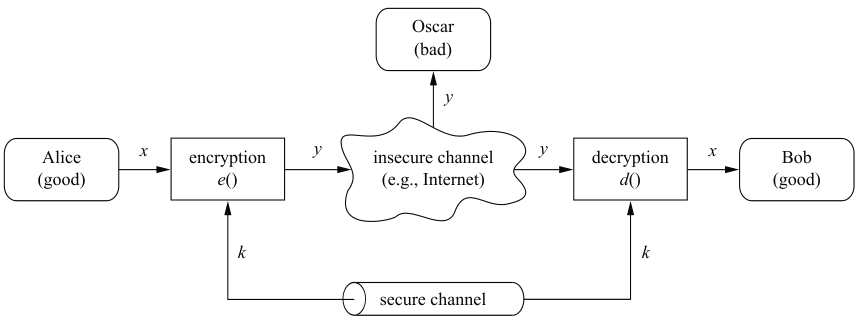
\includegraphics[width=.9\linewidth]{img/sym_alg.png}
\caption{Sơ đồ hệ mật mã Khóa Đối xứng}
\label{fig:sym_alg}
\end{figure}

Sơ đồ \ref{fig:sym_alg} minh họa một ứng dụng mật mã Khóa Đối xứng trong thực tế\cite{10.5555/1721909}. Alice và Bob là 2 người bạn cần trao đổi thông tin bí mật bằng phương pháp sử dụng mật mã Khóa Đối xứng. Trong khi đó Oscar luôn tìm cách giải mật thông tin nghe được giữa Alice và Bob. Nhưng Alice và Bob có được khóa nên liên lạc được, chỉ Oscar thiếu duy nhất khóa để giải mật nên không thể hiểu thông tin.

Các ký hiệu trong sơ đồ \ref{fig:sym_alg}:
\begin{itemize}
\item x là bản rõ
\item y là bản mật
\item k là khóa 
\end{itemize}

\textbf{Mật mã Khóa Bất đối xứng} dùng hai khóa Cá nhân và khóa Công khai trong thuật toán tạo mật mã và giải mật, cặp khóa có liên hệ chặt chẽ nhau về toán học. Khóa Công khai được công bố cho cộng đồng sử dụng nên dễ bị lộ, còn khóa Cá nhân chỉ có cá nhân được sở hữu. Mặc khác khóa Công khai bị lộ thì cũng rất khó (sử dụng Phân tích mật mã) có thể tìm được khóa Cá nhân.
Khóa cá nhân dùng để tạo mật mã và tạo chữ ký số. Khóa công khai dùng để giải mật mã và xác thực chữ ký số. Ví dụ: khi mật mã dùng một khóa công khai thì chỉ có khóa cá nhân của cặp khóa đó mới giải mã được; Tương tự, dùng một khóa cá nhân tạo chữ ký số thì chỉ có khóa công khai tương ứng mới xác thực chữ ký số đó.

\subsection{Hàm băm}

Hàm băm là phép biến đổi một chiều có đầu vào là thông điệp chiều dài bất kỳ thành một dãy bit có độ dài cố định (tùy thuộc vào thuật toán băm). Giá trị băm còn gọi là hash value (hay Digest) là đặc trưng cho thông điệp ban đầu.

Hàm băm là hàm một chiều, theo nghĩa từ giá trị của hàm băm rất khó để suy ngược lại nội dung hay độ dài ban đầu của thông điệp gốc.

Các hàm băm dòng MD: MD2, MD4, MD5 được Rivest đưa ra có kết quả đầu ra với độ dài là 128 bit. Chuẩn hàm băm an toàn: SHA, được Viện Tiêu Chuẩn và Công Nghệ Quốc Gia (NIST) công bố, SHA1 có kết quả đầu ra dài 160bit, SHA2: SHA-256, SHA-384, SHA-512 có kết quả đầu ra dài lần lượt là 256, 384, 512 bit \cite{10.5555/1721909}.

Ví dụ: Với thông điệp ban đầu là Hello world sẽ có các giá trị băm tương ứng với một số hàm băm, như sau:

MD5: 3e25960a79dbc69b674cd4ec67a72c62

SHA-256: 64ec88ca00b268e5ba1a35678a1b5316d212f4f366b2477232\ldots 37f3c

Băm là một giải pháp tạo ra một đặc trưng cho một file dữ liệu. Tương tự như mỗi người có một dấu vân tay đặc trưng. Vì vậy Băm còn được gọi dấu vân tay (Fingerprint) của file dữ liệu.

Hàm băm (Hash Function) là một dạng mật mã tạo bản mật không cần giải mật mà đáp ứng yêu cầu kiểm tra tính toàn vẹn của một dữ liệu dựa trên đặc trưng vân tay của nó \cite{phạmnguyênkhang2013}.

Hàm băm H(x) có khả năng bảo mật tốt, nếu thỏa 3 tính chất: 
Một chiều (One Way),  Tự do liên kết yếu (Weakly Collision Free) và Tự do liên kết mạnh (Strong Collision Free).

\begin{itemize}
\item \emph{Tính chất Một chiều}: Cho trước giá trị băm y, rất khó tìm được x: H(x) = y. Điều này có nghĩa là nhận được giá trị băm y, rất khó tìm được dữ liệu gốc x thỏa: H(x) = y. Tính chất này đảm bảo rất ít tập dữ liệu x có H(x) = y.

\item \emph{Tính chất Tự do liên kết yếu}: cho trước tập dữ liệu x, rất khó tìm được tập dữ liệu x’≠x: H(x)=H(x’). Nếu x là tập dữ liệu cần băm, thì hầu như không thể tìm được tập dữ liệu khác x’: H(x’)=H(x). Tính chất này đảm bảo tệp dữ liệu x kèm H(x) rất khó bị sửa thành x’ có cùng H(x).

\item \emph{Tính chất Tự do liên kết mạnh}: rất khó có thể tìm được 2 tập dữ liệu x ≠ x’ có cùng giá trị băm H(x) = H(x’).
\end{itemize}

\subsection{Chữ ký số}
Chữ ký số được định nghĩa là một loại chữ ký điện tử, được tạo bằng sự chuyển đổi thông điệp dữ liệu sử dụng một hệ thống mật mã không đối xứng, theo đó người có được thông điệp dữ liệu ban đầu và khóa công khai của người ký có thể xác định được chính xác.

\begin{enumerate}[a)]
\item Việc biến đổi nêu trên được tạo ra bằng đúng khóa bí mật tương ứng với khóa công khai trong cùng một cặp khóa;
\item Sự toàn vẹn nội dung của thông điệp dữ liệu kể từ khi thực hiện việc biến đổi nêu trên.
\end{enumerate}

Chữ ký số có chung mục tiêu như chữ ký tay trên văn bản. Chữ ký tay xác định một người bằng dấu vết riêng tác động lên văn bản và qua đó văn bản được ký là chứng cứ sự thật do người đó tạo lập nên. Chữ ký số là thành phần quan trọng trong những giải pháp ứng dụng mật mã, và được áp dụng rộng rãi trong môi trường điện tử đến hiện nay. Chữ ký số cùng với cơ chế trao đổi khóa là cơ sở quan trọng trong hạ tầng khóa công khai. Tuy nhiên, chữ ký số chỉ có thể đảm bảo khi khóa bí mật không bị lộ. Khi khóa bí mật bị lộ thì người sở hữu chữ ký không thể ngăn chặn được việc bị giả mạo chữ ký.

Công nghệ blockchain và chữ ký số cùng đảm bảo thông tin không bị thoái thác. Weidong Fang và cộng sự \cite{Fang2020} nghiên cứu các sơ đồ chữ ký số điển hình trong blockchain gồm các chữ ký số hiện đại nhất được điều tra và so sánh về các lĩnh vực ứng dụng, phương pháp, bảo mật và hiệu suất.
Tuy nhiên, sơ đồ chữ ký số phổ biến hiện nay là sơ đồ chữ ký RSA được Diffie-Hellman đề xuất vào năm 1976 và được Ronald Linn Rivest, Adi Shamir và Leonard Adleman thực hiện vào năm 1977. \cite{10.5555/1721909}. 

Sơ đồ chữ ký số bao gồm 3 thành phần: thuật toán tạo ra khóa, hàm tạo chữ ký và hàm kiểm tra chữ ký.

Hàm tạo ra chữ ký là hàm tính toán chữ ký trên cơ sở khóa mật và dữ liệu cần ký.

Hàm kiểm tra chữ ký là hàm kiểm tra xem chữ ký đã cho có đúng với khóa công cộng không. Khóa này mọi người có quyền truy cập cho nên mọi người đều có thể kiểm tra được chữ ký.

\subsubsection{Nguyên lý ký số và xác thực chữ ký số }

\begin{figure}[htbp]
\centering
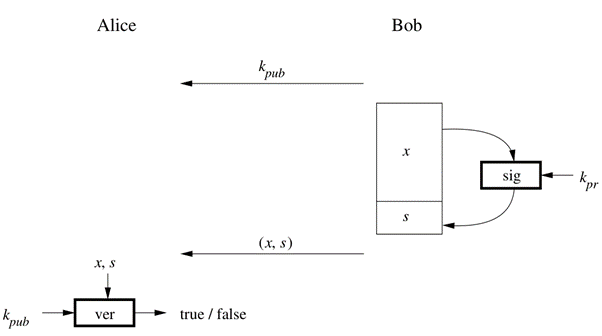
\includegraphics[width=.9\linewidth]{img/dig_sig.png}
\caption{Sơ đồ ký số và xác thực chữ ký số}
\label{fig:dig_sig}
\end{figure}
Sơ đồ nguyên lý ký số và xác thực chữ ký số\cite{10.5555/1721909} được mô tả ở hình ~\ref{fig:dig_sig}.
Quy trình bắt đầu khi Bob ký thông điệp x. Thuật toán ký số (sig) có tham số thứ nhất là khóa bí mật của Bob, $k_{pr}$ . Khóa bí mật được Bob giữ và chỉ anh ta mới có thể ký số lên thông điệp x. Thông điệp x là tham số thứ hai của thuật toán ký số. Sau đó bản chữ ký s sẽ thêm vào thông điêp x tạo một cặp (x,s) gửi cho Alice.
 
Tiếp theo Alice xác minh chữ ký nhận được có hợp lệ hay không. Hàm xác thực (ver) có 2 tham số (x,s) và $k_{pub}$  của Bob. Nếu x do Bob ký số thì được kết quả true, ngược lại false.


Tuy nhiên, với thông điệp x rất lớn thì chữ ký số lớn và ký chậm. Như vậy, thay vì ký số lên thông điệp x, thì có thể ký số lên giá trị băm của x = h(x), giá trị h(x) nhỏ hơn thông điệp x và luôn có chiều dài cố định, đồng nghĩa sẽ nhanh hơn. 

\begin{figure}[htbp]
\centering
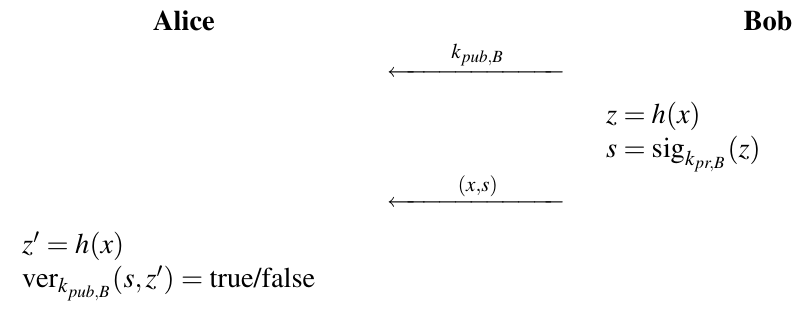
\includegraphics[width=.9\linewidth]{img/dig_sig_hash.png}
\caption{Sơ đồ ký số và xác thực chữ ký số với hàm băm}
\label{fig:dig_sig_hash}
\end{figure}
 Sơ đồ \ref{fig:dig_sig_hash} mô tả nguyên lý ký số và xác thực chữ ký số với hàm băm\cite{10.5555/1721909}.
Bob sẽ tính giá trị băm của thông điệp x và ký số lên giá trị băm z = h(x) bằng khóa bí mật $K_{pr,B}$. Còn bên nhận, Alice sẽ tính giá trị băm z’ của thông điệp x: z’=h(x). Alice sẽ xác thực chữ ký s với khóa công khai $K_{pub,B}$ và z’.

\subsubsection{Chức năng của chữ ký số và tiêu chí an toàn thông tin}
Chữ ký số đảm bảo 2 tiêu chí an toàn thông tin như sau:
\begin{enumerate}
\item Tính toàn vẹn thông tin: khi có sự thay đổi bất kỳ lên thông điệp thì giá trị hàm băm sẽ bị thay đổi; nghĩa là thông điệp không toàn vẹn.
\item Tính không chối bỏ hay chống thoái thác trách nhiệm: vì chỉ có chủ thông điệp mới có khóa bí mật để ký lên thông điệp nên người ký không thể chối bỏ thông điệp của mình.
\end{enumerate}

\subsection{Chứng thư số}

Chứng thư số là một dạng chứng thư điện tử do tổ chức cung cấp dịch vụ chứng thực số (Certification Authority) cấp nhằm cung cấp thông tin định danh cho khóa công khai của một cơ quan, tổ chức, cá nhân, từ đó xác nhận cơ quan, tổ chức, cá nhân là người ký chữ ký số bằng việc sử dụng khóa bí mật tương ứng. 

Chứng thư X.509 phiên bản 3 có những thông tin sau:
\begin{figure}[htbp]
\centering
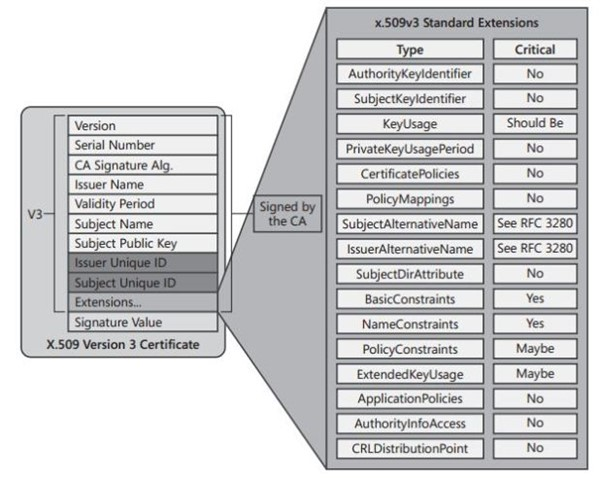
\includegraphics[width=.9\linewidth]{img/x509v3.jpg}
\caption{Cấu trúc chứng thư số X.509 phiên bản 3}
\end{figure}
\begin{itemize}

\item Chủ thể (subject) của chứng thư: thông tin về người dùng, máy tính, thiết bị mạng giữ khóa bí mật tương ứng với chứng thư được cấp phát.
\item Tên dịch vụ chứng thực chữ ký số: thông tin về tổ chức cung cấp chứng thư.
\item Khóa công khai tương ứng với khóa bí mật được liên kết với chứng thư.
\item Tên của các thuật toán để mã hóa và thuật toán tạo chữ ký số cho chứng thư.
\item Trạng thái thu hồi (revocation) và tính hiệu lực của chứng thư (như ngày phát hành và ngày hết hạn).
\item Các phần mở rộng (extension) cho loại chứng chỉ X.509 version 3.

\end{itemize}

Phân loại chứng thư số

\begin{itemize}
\item \emph{Chứng thư số tổ chức} là chứng thư số dùng để nhận diện các chủ thể là các tổ chức trên môi trường điện tử. Chữ ký số tạo bởi chứng thư số này có giá trị pháp lý như con dấu của tổ chức.
\item \emph{Chứng thư số cá nhân} là chứng thư số dùng để nhận diện các cá nhân trên môi trường điện tử. Chữ ký số tạo bởi từ chứng thư số cá nhân có giá trị pháp lý như chữ ký tay của cá nhân khi thực hiện các giao dịch. Chữ ký số tạo bởi từ chứng thư số này có giá trị pháp lý như chữ ký tay của cá nhân khi thực hiện các giao dịch điện tử
\item \emph{Chứng thư số cá nhân thuộc tổ chức} là chứng thư số dùng để nhận diện chủ thể là các cá nhân thuộc các tổ chức trên môi trường điện tử. Chữ ký số tạo bởi chứng thư số này có giá trị pháp lý như chữ ký tay của cá nhân trong tổ chức. Chứng thư số này thường gắn với các chức danh nội bộ của chủ thể như: Tổng giám đốc, Giám đốc, Trưởng phòng, kế toán trưởng…
\end{itemize}

\subsection{Dịch vụ chứng thực số}
Dịch vụ chứng thực số là một loại hình dịch vụ chứng thực chữ ký số, do tổ chức cung cấp dịch vụ chứng thực chữ ký số cung cấp cho thuê bao để xác thực việc thuê bao là người đã ký số trên thông điệp dữ liệu. 

Dịch vụ chứng thực chữ ký số bao gồm: 

\begin{itemize}
\item Tạo cặp khóa hoặc hỗ trợ tạo cặp khóa bao gồm khóa công khai và khóa bí mật cho thuê bao;
\item Cấp, gia hạn, tạm dừng, phục hồi và thu hồi chứng thư số của thuê bao; 
\item Duy trì trực tuyến cơ sở dữ liệu về chứng thư số; 
\item Cung cấp thông tin cần thiết để giúp chứng thực chữ ký số của thuê bao đã ký số trên thông điệp dữ liệu.
\end{itemize}

\subsection {Hạ tầng khóa công khai}
Hạ tầng khóa công khai (Public Key Infrastructure) là một cơ chế để cho một bên thứ ba (thường là nhà cung cấp chứng thực số) cung cấp và xác thực danh tính các bên tham gia vào quá trình trao đổi thông tin. Cơ chế này cũng cho phép gán cho mỗi người sử dụng trong hệ thống một cặp khóa công khai/khóa riêng tư. Các quá trình này thường được thực hiện bởi một phần mềm đặt tại trung tâm và các phần mềm khác tại các địa điểm của người dùng. Khóa công khai thường được phân phối trong hạ tầng khóa công khai.

Khái niệm hạ tầng khóa công khai PKI thường được dùng chỉ toàn bộ hệ thống bao gồm cả nhà cung cấp chứng thực số (CA) cùng các cơ chế liên quan đồng thời với toàn bộ việc sử dụng các thuật toán mã hóa công khai trong trao đổi thông tin. Tuy nhiên, các cơ chế trong PKI không nhất thiết sử dụng các thuật toán mã hóa công khai.

\section{Công nghệ Blockchain}
\subsection{Giới thiệu}
Blockchain là cuốn sổ cái kỹ thuật số chống giả mạo được triển khai theo mô hình phân tán (không có kho lưu trữ trung tâm), còn gọi là công nghệ sổ cái phân tán (Decentralized Ledger Technology).
Khi người dùng phát sinh các giao dịch, sau khi được cộng đồng chấp nhận ghi vào sổ cái thì giao dịch đó không thể bị thay đổi.
Công nghệ này được biết đến rộng rãi vào năm 2009 với sự ra đời của mạng Bitcoin\cite{nakamoto2008bitcoin}, một trong những đồng tiền mã hóa hiện đại đầu tiên được bảo vệ bởi các cơ chế mật mã học thay vì nhờ vào bên chứng thực hoặc kho lưu trữ trung tâm.

\textbf{Phân loại Blockchain}

Mạng Blockchain có thể được phân loại thành: Blockchain công khai và Blockchain riêng tư \cite{8246573}. 
Loại thứ nhất gồm Bitcoin, Ethereum, \ldots, bất kỳ nút nào cũng có thể tham gia và rời khỏi mạng Blockchain, mô hình này phân tán hoàn toàn, mỗi nút có vai trò như nhau.
Loại thứ hai gồm Hyperledger, BigchainDB, Ripple, Parity,\ldots, việc tham gia mạng Blockchain được kiểm soát chặt chẽ, xác định rõ danh tính của thành viên.

\textbf{So sánh giữa các mạng Blockchain}

Tien Tuan Anh Dinh và cộng sự  \cite{8246573} nghiên cứu và so sánh mạng Blockchain dựa trên 4 khái niệm chính của Blockchain: sổ cái phân tán, cơ chế đồng thuận (concensus), mô hình ứng dụng mật mã, hợp đồng thông minh (smart contract),

\emph{Sổ cái phân tán}

Blockchain không dựa vào các tổ chức thứ ba để xử lý giao dịch, không có sự kiểm soát trung tâm.
Tất cả thông tin được các nút kiểm tra, truyền tải và quản lý. 
Các nút lưu trữ bản sao của sổ cái, gồm các giao dịch trong từng khối ghép nối với nhau thành chuỗi.
Cơ chế sổ cái phân tán là đặc điểm nổi bật và quan trọng nhất của Blockchain.
Khái niệm sổ cái phân tán có 3 tiêu chí phân loại được mô tả ở bảng \ref{table:ex-dlt} 
\begin{table}
\caption{So sánh sổ cái phân tán}
	\label{table:ex-dlt}
	\begin{tabularx} {\textwidth} {|X|X|X|p{5cm}|}
\hline
	Dữ liệu mô tả & Số lượng sổ & Quyền kiểm soát & Ứng dụng \\ \hline
	Tài khoản  & 1 & Người quản trị & Số cái thông thường với hình thức lưu trữ tập trung ở những ngân hàng\\ \hline
	Tài sản   & Nhiều  &  Nhiều người & Số cái riêng của một tổ chức hoặc nhóm các tổ chức\\ \hline
	Tiền hoặc tài khoản   &  1 & Bất cứ người nào & Lĩnh vực tiển số: Bitcoin, Ethereum \\ \hline
\end{tabularx}
\end{table}

\emph{Cơ chế đồng thuận}

Trong Blockchain, sổ cái lưu trữ toàn bộ lịch sử các giao dịch và trạng thái dữ liệu hiện tại.
Để sổ cái được lưu trữ, cập nhật dữ liệu giống nhau ở tất cả các nút thì cần có sự thống nhất giữa các bên tham gia. Ngược lại việc một tổ chức có đặc quyền cập nhật dữ liệu trong các ứng dụng CSDL truyền thống.
Tuy nhiên, Blockchain không phụ thuộc vào độ tin cậy của một nút. Các nút không tin cậy như bài toán các vị tướng Byzantine. Do đó các nút sẽ yêu cầu thực hiện giải thuật đồng thuận để có chung một quyết định.
Cơ chế đồng thuận hiện nay có thể chia thành ba loại \cite{lequyetthang2016}

(1) POW (Proof of Work) là cơ chế của Bitcoin:
Cơ chế này yêu cầu các nút tính toán đề xuất khối mới và được đa số nút kiểm tra thành công tính tin cậy của các giao dịch phát sinh trong khối. Đối với Bitcoin, POW mật độ giao dịch (năm 2008) là 7 giao dịch/giây dẫn đến trung bình 10 phút xác thực thành công 1 khối. 

(2) PBFT (Practical Byzantine Fault Tolerance): mỗi thành viên tạo khối mới của mình, kiểm tra xong thì chuyển cho thành viên khác kiểm tra, đồng thời nhận khối mới từ thành viên khác để kiểm tra. Khối nào được đa số chấp nhận thì được chọn đưa vào blockchain. 
Cơ chế này được dùng trong mạng Blockchain riêng tư bởi các nút đã xác định danh tính.

(3) POS (Proof of Stake): Mỗi thành viên tham gia mạng có một cổ phần (Stake) với một lượng lớn hay nhỏ tùy đầu tư ban đầu. Đầu tư càng cao thì trách nhiệm càng cao. Trách nhiệm càng cao thì khả năng kiểm tra một giao dịch đúng càng cao. 

\emph{Mô hình ứng dụng mật mã}

Blockchain ứng dụng mật mã khóa công khai. Khi giao dịch phát sinh, khóa công khai và chữ ký sẽ được dùng để kiểm tra danh tính.
Khi thực hiện mã hóa giao dịch thì khóa công khai, chữ ký và thông tin người dùng của giao dịch trước đó phải khớp nhau.

Do đó thuộc tính khóa có vai trò quan trọng để xác định danh tính và xác minh giao dịch, nên cần được giữ an toàn. Trong những ứng dụng Blockchain vào tiền số, nếu xảy ra sự cố mất khóa thì gây thiệt hại thất thoát tiền, vì không thể khôi phục, xử lý dữ liệu của Blockchain.
Ngược lại trong Blockchain riêng tư, thành phần quản lý cấp phép truy cập tách biệt với mã hóa giao dịch. Đối với Hyperledger, các dịch vụ chứng thực số và dịch vụ thành viên (Membership Service Provider) sẽ cấp phép truy cập, nên một tài khoản quản lý thuộc tổ chức sẽ có quyền thiết lập cấp phép những dịch vụ, người dùng được truy cập vào mạng Blockchain.

\emph{Hợp đồng thông minh}



\begin{table}
\caption{So sánh các Blockchain}
	\label{table:ssblochchain}
	\begin{tabularx} {\textwidth} {|X|X|X|X|}
\hline
	Blockchain & Thực thi HĐTM & Ngôn ngữ HĐTM  & Dữ liệu mô tả \\ \hline
	Bitcoin  & Thuộc ứng dụng & Go, C++ & Giao dịch\\ \hline
	Ethereum  & EVM & Solidity, Serpent, LLL, C++ & Giao dịch\\ \hline
	Hyperledger Farbic v1.x  & Dockers & Go, Java & Khóa-Giá trị\\ \hline
	BigchainDB   & Thuộc ứng dụng  &  Python & Giao dịch\\ \hline
	Ripple   & -  & - & Tài khoản \\ \hline
\end{tabularx}
\end{table}

\subsection{Bitcoin}
Mạng Bitcoin gồm có thành phần miner và Blockchain.

Miner là một node trên mạng kết nối với nhau theo giao thức mạng ngang hàng.
Miner kết nối người dùng trong mạng và Blockchain.
Bitcoin cho phép phát hành tiền mới thông qua cơ chế ``phần thưởng" cho miner sau khi khối của mình tạo ra được xác thực hợp lệ. Cơ chế đồng thuận để duy trì và tự kiểm soát để đảm bảo rằng chỉ có các giao dịch và các khối hợp lệ mới được thêm vào Blockchain.

Blockchain là một hệ thống cơ sở dữ liệu phân tán lưu trữ các khối liên kết với nhau sau khi đã xác thực thành công bởi các miner. Hình \ref{fig:merkle_bitcoin} mô tả cấu trúc một khối bao gồm các thành phần: định danh khối (blockheader) và dữ liệu.
Blockheader là giá trị băm của các thành phần gồm: Root hash của các dữ liệu giao dịch, giá trị blockheader của khối trước, số thứ tự khối, số nounce, nhãn thời gian.

\begin{figure}[htbp]
\centering
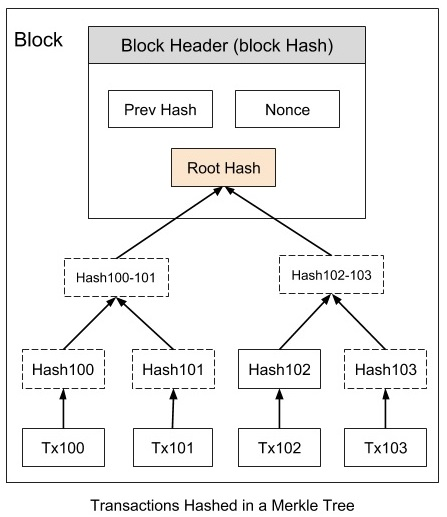
\includegraphics[width=.5\linewidth]{img/merkle_tree.jpg}
\caption{Mô tả cấu trúc một khối}
\label{fig:merkle_bitcoin}
\end{figure}

Một dữ liệu giao dịch gồm có nhiều giao dịch được ký số bởi các bên tham gia như hình \ref{fig:trans_bitcoin}.

\begin{figure}[htbp]
\centering
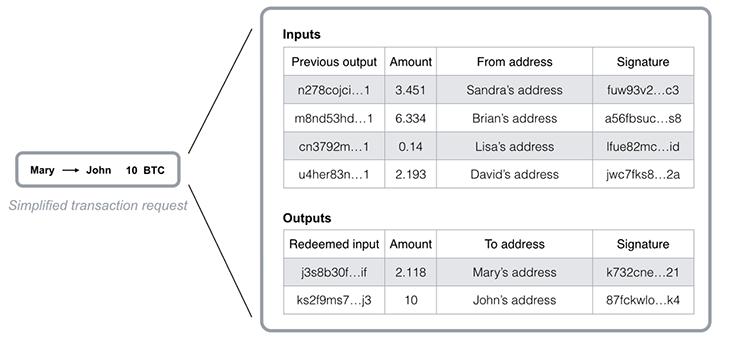
\includegraphics[width=.9\linewidth]{img/trans_bitcoin.png}
\caption{Mô tả một giao dịch blockchain}
\label{fig:trans_bitcoin}
\end{figure}

Mỗi dữ liệu giao dịch A, B, C, D, E được tính giá trị băm, sau đó gộp 2 khối dữ liệu thành từng cặp, tính giá trị băm trung gian, công việc này lặp lại cho đến khi tính được giá trị băm các giao dịch (Root Hash) được mô tả như hình \ref{fig:merkle}. 

\begin{figure}[htbp]
\centering
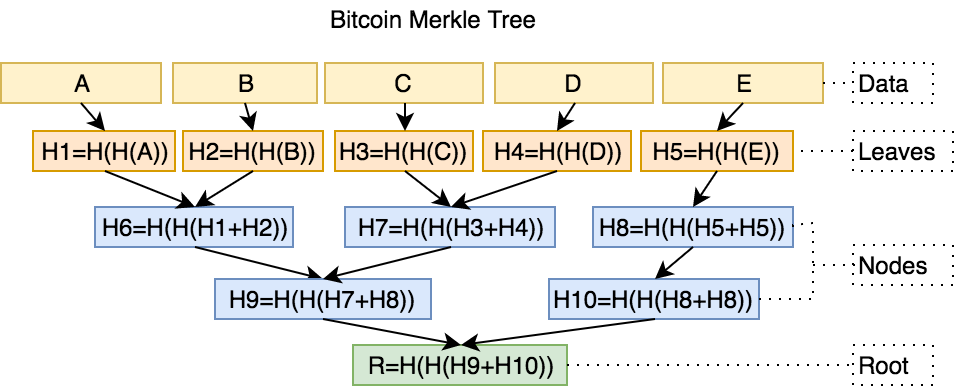
\includegraphics[width=.9\linewidth]{img/merkle.png}
\caption{Mô tả cây mã hóa Merkle trong Bitcoin}
\label{fig:merkle}
\end{figure}

Giao dịch trong Blockchain có thể chia thành 3 loại: giao dịch  thuộc về khối đầu tiên của Blockchain, giao dịch thưởng cho các miner và giao dịch thông thường.

\begin{itemize}
\item Giao dịch thuộc về khối đầu tiên của Blockchain sẽ được chèn vào trong mã nguồn của Blockchain tại khối đầu tiên của Blockchain. Các loại tiền số có quy định số lượng tiền giới hạn trong hệ thống.
\item Giao dịch thưởng cho những người tạo ra khối mới: hệ thống Blockchain tự tạo tự động và sẽ chuyển tiền thưởng cho người tạo ra khối mới.
\item Giao dịch thông thường là những giao dịch được tạo bởi những người dùng. 
\end{itemize}

Mạng Bitcoin và các hệ thống Blockchain tương tự, việc chuyển thông tin kỹ thuật số với đại diện là tiền điện tử diễn ra trong một hệ thống phân tán.
Người dùng Bitcoin ký chữ ký số và chuyển tài sản của mình sang người khác và Bitcoin ghi lại các giao dịch này công khai, cho phép những người tham gia mạng xác minh độc lập tính hợp lệ của giao dịch. 
Do đó, công nghệ blockchain được xem là giải pháp chung cho các đồng tiền mã hóa sau này.

\subsection{Ethereum}

\subsection{Bigchaindb}

\subsection{Hyperledger Fabric}

\textbf{Giới thiệu}

Hyperledger Fabric là một nền tảng blockchain trong dự án Hyperledger của tổ chức Linux Foundation gồm: Hyperledger Indy, Hyperledger Fabric, Hyperledger Iroha, Hyperledger Sawtooth, Hyperledger Burror. Hình \ref{fig:hlf_um} mô tả dự án Hyperledger.

Hyperledger Fabric thuộc nhóm phần mềm mã nguồn mở dưới sự cố vấn của công ty IBM. Mục đích thiết kế Hyperledger Fabric là cung cấp rộng rãi nền tảng ứng dụng blockchain cho các tổ chức, doanh nghiệp. Hyperledger Fabric có nhiều tính năng nổi trội so với các nền tảng blockchain phổ biến như Bitcoin, Ethereum. Hyperledger Fabric có kiến trúc mô-đun linh hoạt và tối ưu hoá cho nhiều ứng dụng trong các lĩnh vực như: tài chính, bảo hiểm, y tế, chuỗi cung ứng, hành chính công, \ldots{}

\begin{figure}[htbp]
\centering
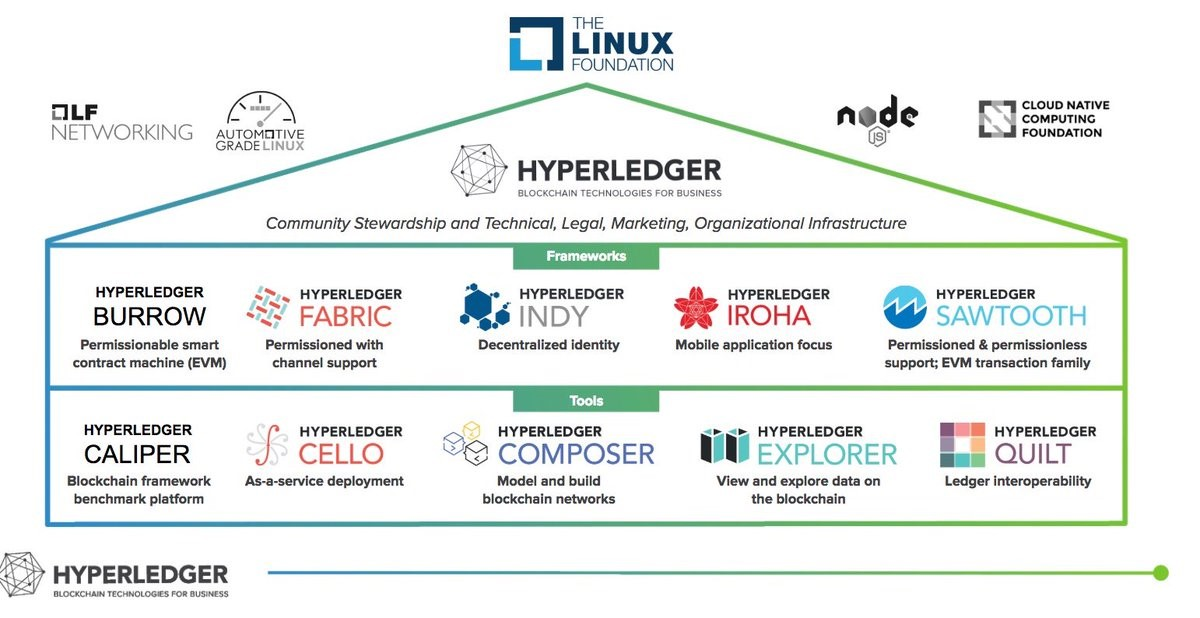
\includegraphics[width=.9\linewidth]{img/hlf_um.jpg}
\caption{Dự án Hyperledger}
\label{fig:hlf_um}
\end{figure}

Nhờ vào thiết kế mô-đun linh hoạt và quản lý người tham gia nên Hyperledger Fabric trở thành nền tảng blockchain có tốc độ xử lý giao dịch nhanh và phù hợp với tổ chức muốn kiểm soát danh tính người tham gia, và xác minh các giao dịch với hợp đồng thông minh.

Phiên bản mới nhất của Hyperledger Fabric là 2.x. Hyperledger Fabric được cộng đồng hỗ trợ các vấn đề bảo mật, cập nhật. Hệ thống sẽ được cập nhật cho đến khi một phiên bản LTS mới được phát hành.

Trong phiên bản Fabric 2.x, các hợp đồng thông minh (smart contract) được cài đặt trên các peer tham gia chung channel và được đánh số các phiên bản. Các tổ chức thuộc kênh (channel) đồng ý các tham số của hợp đồng thông minh, chứng thực hợp đồng thông minh sau đó hợp đồng thông minh mới thực hiện tương tác với sổ cái (ledger).

Việc nâng cấp các hợp đồng thông minh (smart contract) sẽ được gắn với quá trình đồng thuận và được các nút mạng đồng ý. Khi đó các peer có đầy đủ các hợp đồng thông minh (chaincode được cài đặt). Việc thay đổi cơ chế nâng cấp hợp đồng thông minh trên phiên bản 2.x mang lại tính an toàn, đồng nhất dữ liệu so với phiên bản trước.

Dữ liệu riêng tư (Data Privacy) cho phép một phần dữ liệu được chia sẽ riêng tư giữa một số thành viên thuộc kênh thay vì tất cả thành viên đều có thể sở hữu. Thay vì tạo thêm một kênh để nhóm các thành viên và mất rất nhiều thời gian để cấu hình (kênh, chính sách, MSP,…) 

Hyperledger Fabric 2.x có hiệu suất xử lý giao dịch đến hàng nghìn giao dịch mỗi giây. Một trong những điểm nổi bật của phiên bản Fabric 2.x là tối ưu hóa hiệu suất hoạt động của mạng Blockchain. Các giải thuật đồng thuận gồm có: Kafka, Raft. Các thực giao dịch được xử lý song song, xử lý khối bất động bộ, phân trang chaincode,\ldots.

\textbf{Các thành phần của Hyperledger Fabric}

\begin{figure}[htbp]
\centering
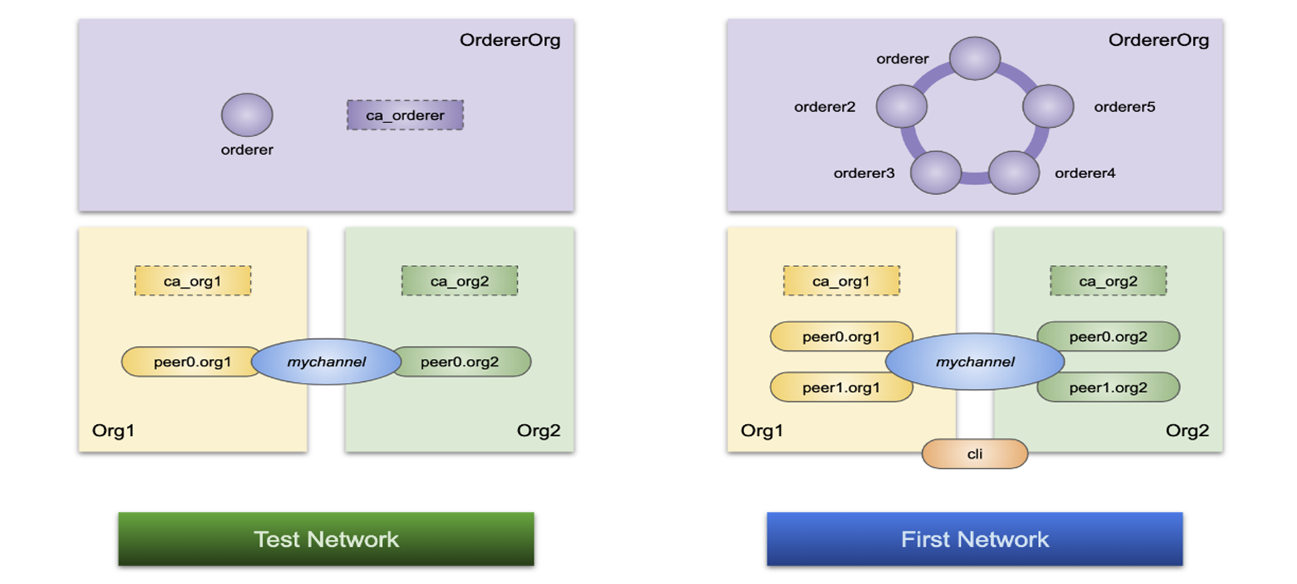
\includegraphics[width=.9\linewidth]{img/hlf_network.png}
\caption{Kiến trúc mạng Hyperledger Fabric}
\label{fig:hlf_network}
\end{figure}

\textbf{Ledger}: Một quyển sổ cái bao gồm 2 thành phần có liên quan nhau là “chuỗi khối” và “cơ sở dữ liệu trạng thái”. Các giao dịch thay đổi các tài sản (dữ liệu trong mạng blockchain) của mạng sẽ được “chuỗi khối” ghi nhận theo dạng nhật ký và không thể xóa hay chỉnh sửa. Ngược lại, “cơ sở dữ liệu trạng thái” (cơ sở dữ liệu LevelDB hoặc CouchDB) lưu trạng thái mới nhất của các tài sản hiện có trong mạng theo cặp khóa-giá trị (key-value). Toàn bộ ledger được lưu trên các Peer trong cùng Channel, và dữ liệu được đồng bộ khi có phát sinh giao dịch thông qua cơ chế đồng thuận.

\textbf{Smart contract} (Chaincode): Hợp đồng thông minh trong blockchain là các ứng dụng được lập trình bằng ngôn ngữ lập trình như: Javascript, Go, Java. Hợp đồng thông minh tương tác với mạng, quản lý tài sản. Trong Hyperledger Fabric, các hợp đồng thông minh còn được gọi là chaincode, được cài đặt trên các Peer.

\textbf{Peer nodes}: Là những nút cơ bản của mạng có chức năng lưu trữ bản sao của Ledgers và thực thi Hợp đồng thông minh. Các peer được quản lý và duy trì bởi các thành viên trong mạng. Peer được chia làm 2 dạng:

\begin{itemize}
\item \textbf{Endorsing peer}: thực thi các giao dịch trong chaincode và đề xuất giao dịch.
\item \textbf{Committing peer}: có thể không cần cài đặt chaincode, lưu trữ sổ cái đầy đủ.
\end{itemize}

\textbf{Ordering Service (Solo, Raft, Kafka)}: Là những nút chứa thuật toán đồng thuận và đảm nhận nhiệm vụ xác minh, bảo mật, kiểm định phân quyền, quản lý cấu hình Channel.

\textbf{Channel}: Kênh là một “mạng con” riêng kết nối giữa hai hoặc nhiều nút trong mạng blockchain. Mỗi kênh sẽ kết nối các nút như Orgs(tổ chức), Peer, Ordering service, MSP. Mỗi Peer có thể tham gia nhiều kênh và sẽ được cấp các định danh riêng với từng kênh bởi dịch vụ xác thực thành viên (MSP).

\textbf{Fabric Certificate Authorities}: Hyperledger Fabric CA là thành phần phát hành chứng thư số. Chứng thư số được cấp dựa trên hạ tầng khóa công khai PKI cho các nút trong mạng và người dùng. CA phát hành một chứng thư gốc (rootCert) cho mỗi thành viên và một chứng nhận đăng ký (ECert) cho mỗi người dùng được uỷ quyền.

\textbf{Membership Service Provider (MSP)}: MSP là dịch vụ xác minh các nút trong mạng, thông qua chứng thư số (cấp từ CA). Do đó HyperLedger Fabric có thể xác thực các thực thể kết nối với mạng thông qua danh tính (Identities) mà không cần khóa bí mật. Ngoài ra, nó còn có vai trò xác định quyền truy cập trong phạm vi mạng và kênh của một thành phần nào đó trong mạng.

\textbf{Bổ kiến trúc xử lý giao dịch}

\textbf{Thiết lập mạng Hyperledger Fabric}

